\documentclass[a4paper,10pt,fleqn]{scrartcl}
\usepackage[utf8]{inputenc}
\usepackage[T1]{fontenc}
\usepackage{amssymb,amsmath}
\usepackage{graphicx}

\date{}
\title{Algorithm development draft on angular-dependent backprojection}

  \numberwithin{equation}{subsection}

\begin{document}
\maketitle\newpage
\section{General algorithm notes}
\textbf{Complexity:}
\begin{equation*}
\mathcal{O}(x^3)
\end{equation*}
\section{Partial pixel effect calculation}
\subsection{Point coordinate calculation}
\begin{minipage}{\textwidth}
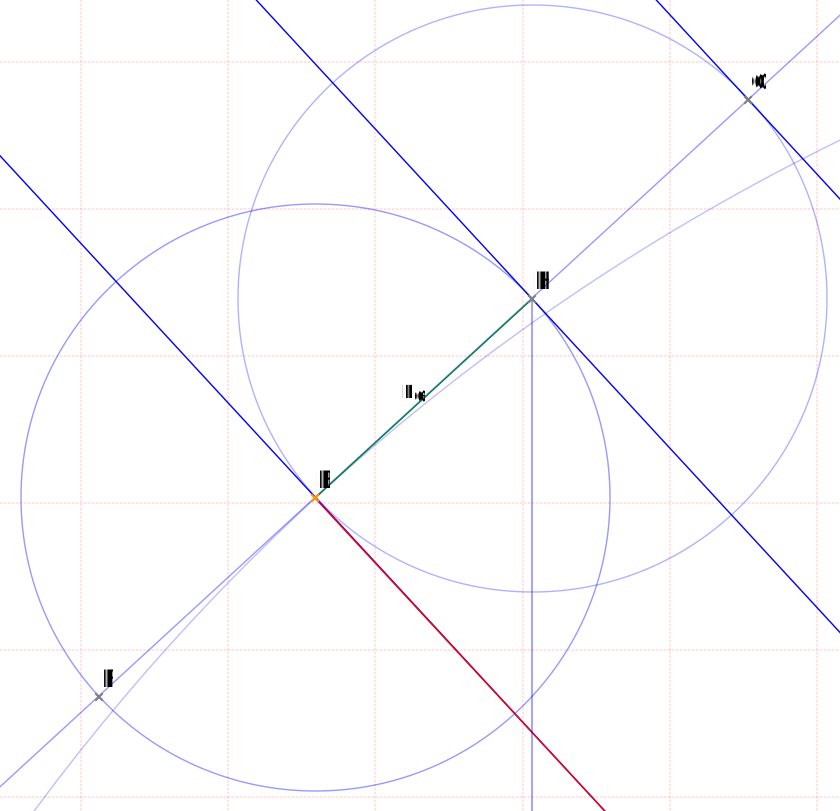
\includegraphics[width=\textwidth]{mappicschema}
\end{minipage}\\
\textrm{Note: All coordinares are relative to M}\\
\begin{align}
E &= (r * cos(\alpha) | r * sin(\alpha)) \\
%\delta &= 90^\circ - \alpha \\
\begin{split}
G &= (x_E + r_e * \sin(\delta) | y_E + r_e * \cos(\delta)) \\
  &= (r * \cos(\alpha) + r_e * \sin(\delta) | r * \sin(\alpha) + r_e * cos(\delta))\\
  &= (r * \cos(\alpha) + r_e * \sin(90^\circ - \alpha) | r * \sin(\alpha) + r_e * cos(90^\circ - \alpha))\\
  &= (r * \cos(\alpha) + r_e * \cos(\alpha) | r * \sin(\alpha) + r_e * \sin(\alpha))\\
  &= ([r + r_e] * \cos(\alpha) | [r + r_e] * \sin(\alpha))
\end{split}\\
\overline{D\,H_D} &= (y_E - y_D) * \tan(90^\circ-\alpha) - x_G - x_D \\
\overline{A\,H_A} &= (y_E - y_A) * \tan(90^\circ-\alpha) - x_G - x_A
%A_E = \frac{1}{2} \overline{D\,H_D} + \overline{A\,S_A} %Effect Amount
\end{align}
\newpage
%
\subsection{Case 1:}
\begin{minipage}{\textwidth}
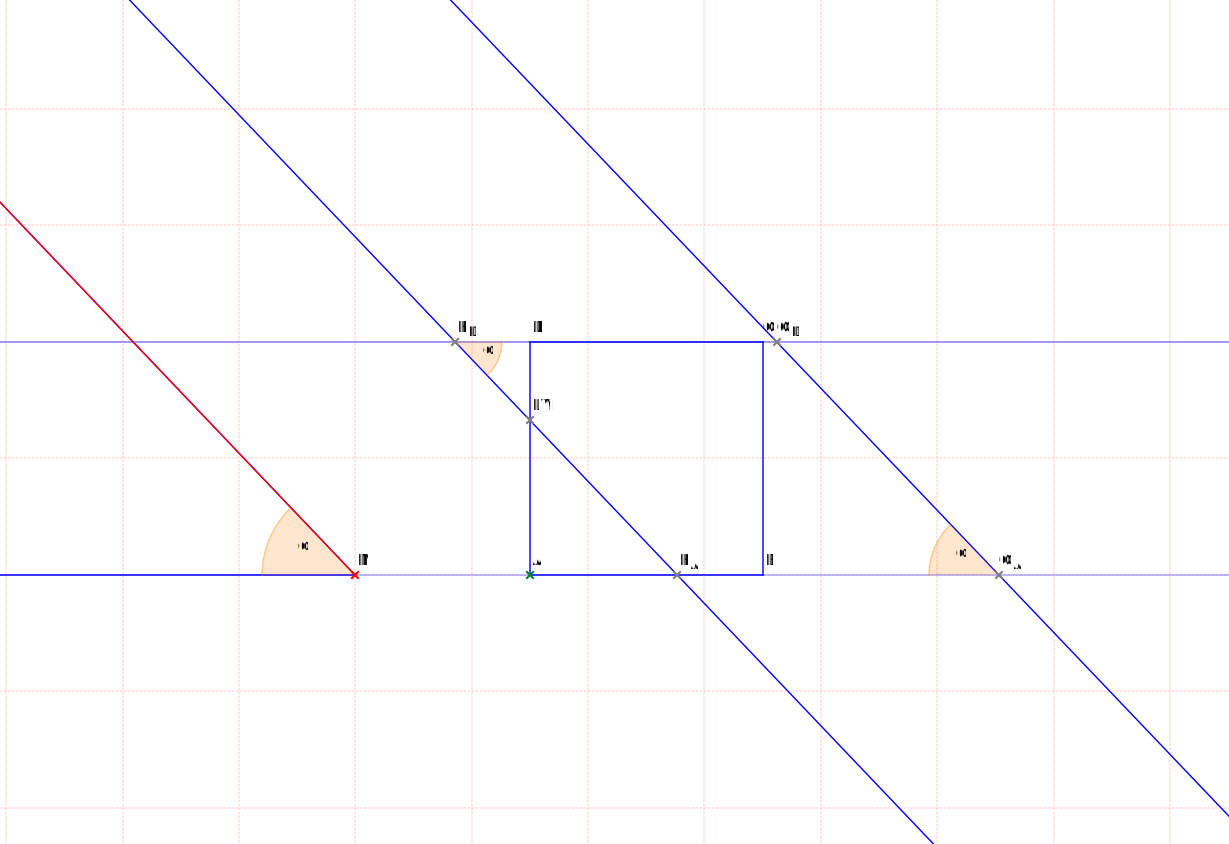
\includegraphics[width=\textwidth]{case1}
\end{minipage}
\begin{align}
Effect &= 1 - (\overline{A\,LVI} * \overline{A\,H_A})\\
\overline{A\,LVI} &=  1 - \tan(\alpha) * \overline{H_D\,D}
\end{align}
\paragraph{Criteria:}
\begin{itemize}
 \item $G_D$ is on the right outside of the pixel
 \item $G_A$ is on the right outside of the pixel
 \item $H_D$ is on the left outside of the pixel
 \item $H_A$ is inside of the pixel
\end{itemize}
%
\subsection{Case 2:}
\begin{minipage}{\textwidth}
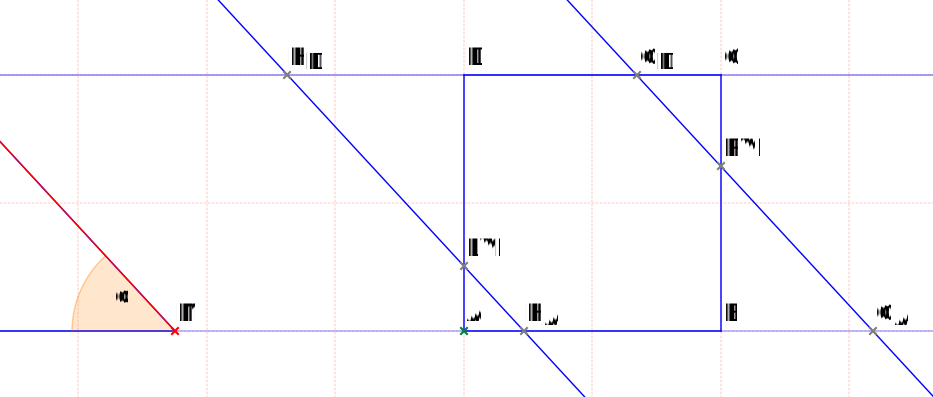
\includegraphics[width=\textwidth]{case2}
\end{minipage}
\begin{align}
Effect &= 1 - (\frac{1}{2} * \overline{C\,RVI} * \overline{G_D\,C} + \frac{1}{2} * \overline{A\,LVI} * \overline{A\,H_A})\\
\overline{C\,RVI} &=  1 - \tan(\alpha) * \overline{B\,G_A}\\
\overline{A\,LVI} &=  1 - \tan(\alpha) * \overline{H_D\,D}
\end{align}
\paragraph{Criteria:}
\begin{itemize}
 \item $G_D$ is inside of the pixel
 \item $G_A$ is on the right outside of the pixel
 \item $H_D$ is on the left outside of the pixel
 \item $H_A$ is inside of the pixel
\end{itemize}
%
\subsection{Case 3:}
\begin{minipage}{\textwidth}
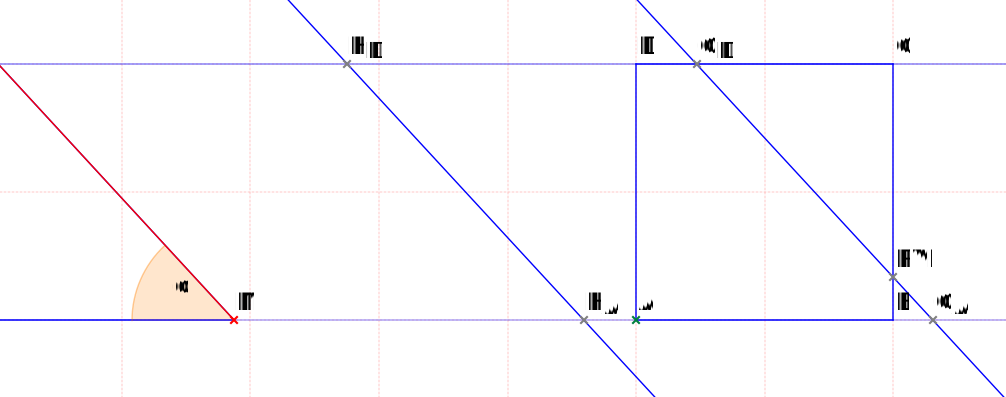
\includegraphics[width=\textwidth]{case3}
\end{minipage}
\begin{align}
Effect &= 1 - (\frac{1}{2} * \overline{C\,RVI} * \overline{G_D\,C})\\
\overline{C\,RVI} &=  1 - \tan(\alpha) * \overline{B\,G_A}
\end{align}
\paragraph{Criteria:}
\begin{itemize}
 \item $G_D$ is on the right outside of the pixel
 \item $G_A$ is on the right outside of the pixel
 \item $H_D$ is on the left outside of the pixel
 \item $H_A$ is on the left outside of the pixel
\end{itemize}
%
\subsection{Case 4:}
\begin{minipage}{\textwidth}
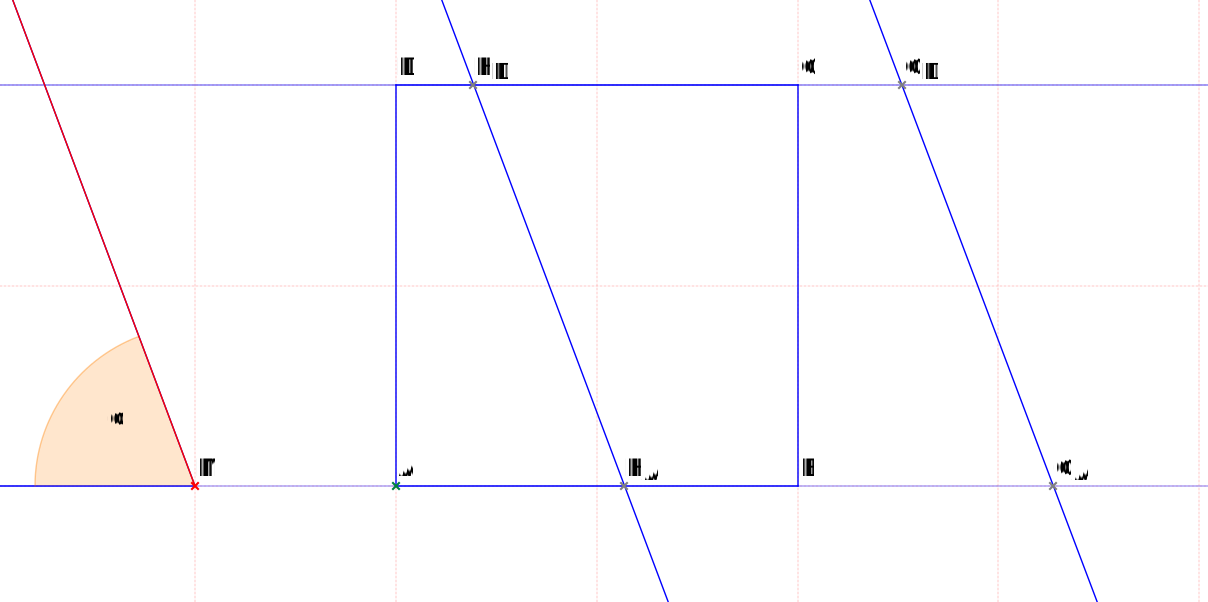
\includegraphics[width=\textwidth]{case4}
\end{minipage}
\begin{align}
Effect &= 1 - (\frac{1}{2} * \overline{C\,RVI} * \overline{G_D\,C})\\
\overline{C\,RVI} &=  1 - \tan(\alpha) * \overline{B\,G_A}
\end{align}
%
\paragraph{Criteria:}
\begin{itemize}
 \item $G_D$ is on the right outside of the pixel
 \item $G_A$ is on the right outside of the pixel
 \item $H_D$ is on the left outside of the pixel
 \item $H_A$ is on the left outside of the pixel
\end{itemize}
%
\subsection{Case 5:}
\begin{minipage}{\textwidth}
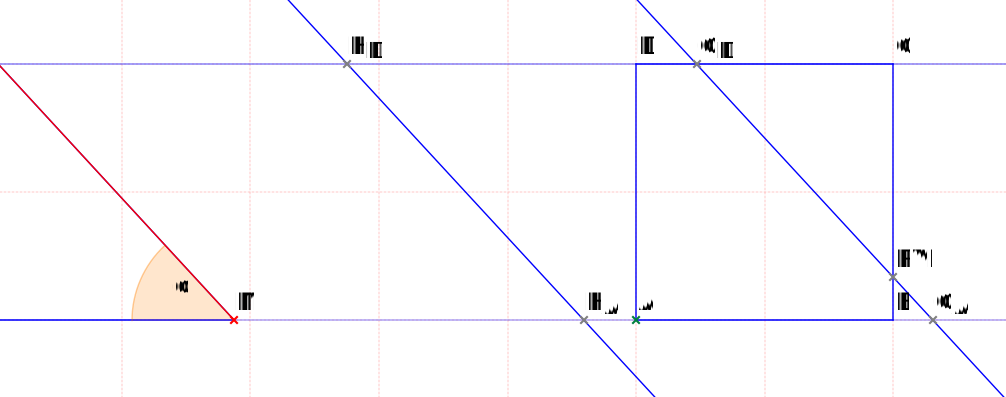
\includegraphics[width=\textwidth]{case3}
\end{minipage}
\begin{align}
Effect &= 1 - (\frac{1}{2} * \overline{C\,RVI} * \overline{G_D\,C})\\
\overline{C\,RVI} &=  1 - \tan(\alpha) * \overline{B\,G_A}
\end{align}
\paragraph{Criteria:}
\begin{itemize}
 \item $G_D$ is on the right outside of the pixel
 \item $G_A$ is on the right outside of the pixel
 \item $H_D$ is on the left outside of the pixel
 \item $H_A$ is on the left outside of the pixel
\end{itemize}
\end{document}